\documentclass[border=12pt]{standalone}
\usepackage{tikz}
\usetikzlibrary{shapes.geometric, arrows.meta, positioning, calc, fit, backgrounds}
\usepackage{fontspec}
\setmainfont{DejaVu Sans}

\begin{document}
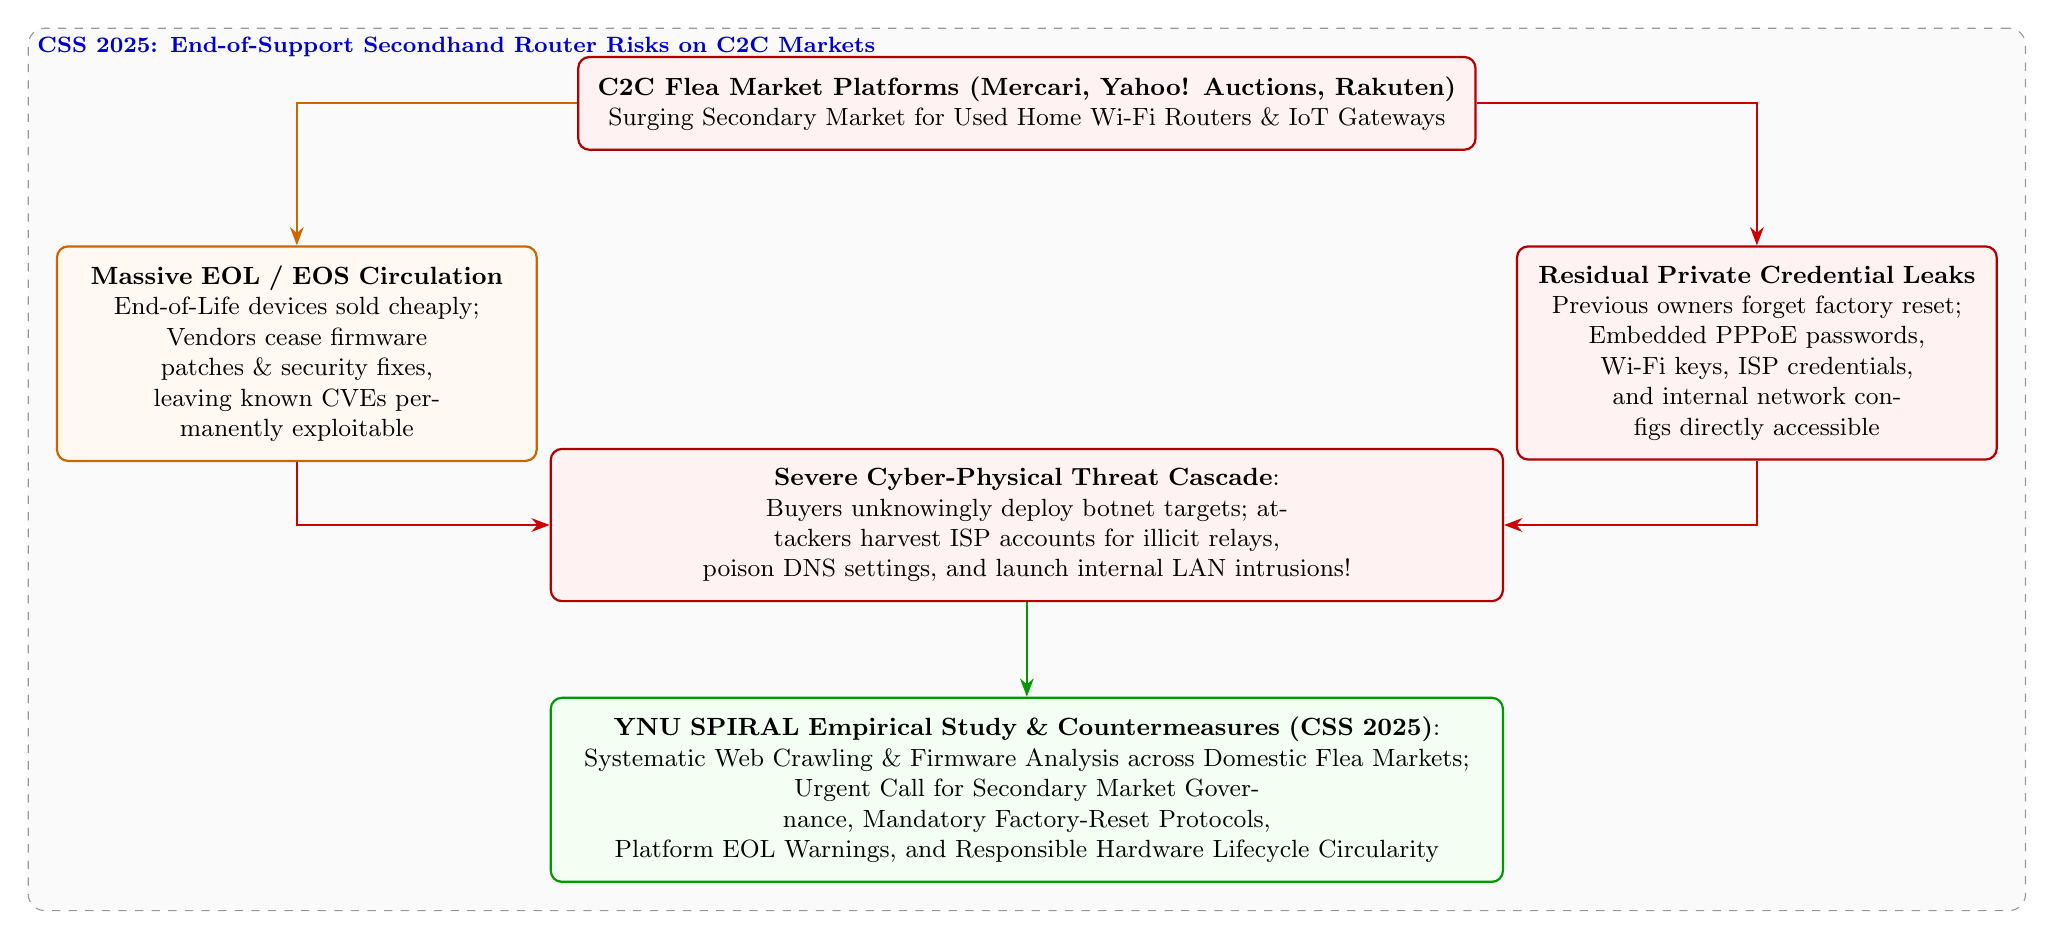
\begin{tikzpicture}[
    font=\small,
    >=Stealth,
    node distance=1.2cm,
    block/.style={rectangle, draw=blue!70!black, fill=blue!5, rounded corners=4pt, thick, align=center, inner sep=7pt},
    alertblock/.style={rectangle, draw=red!70!black, fill=red!5, rounded corners=4pt, thick, align=center, inner sep=7pt},
    greenblock/.style={rectangle, draw=green!60!black, fill=green!5, rounded corners=4pt, thick, align=center, inner sep=7pt},
    amberblock/.style={rectangle, draw=orange!80!black, fill=orange!5, rounded corners=4pt, thick, align=center, inner sep=7pt},
    groupbox/.style={draw=black!40, dashed, rounded corners=6pt, fill=black!2, inner sep=10pt}
]

    % Top Problem
    \node[alertblock] (market) {\textbf{C2C Flea Market Platforms (Mercari, Yahoo! Auctions, Rakuten)}\\Surging Secondary Market for Used Home Wi-Fi Routers \& IoT Gateways};

    % Two Threat Realities
    \node[amberblock, below left=1.2cm and 0.5cm of market, text width=5.6cm] (eol) {\textbf{Massive EOL / EOS Circulation}\\End-of-Life devices sold cheaply;\\Vendors cease firmware patches \& security fixes,\\leaving known CVEs permanently exploitable};

    \node[alertblock, below right=1.2cm and 0.5cm of market, text width=5.6cm] (residual) {\textbf{Residual Private Credential Leaks}\\Previous owners forget factory reset;\\Embedded PPPoE passwords, Wi-Fi keys, ISP credentials,\\and internal network configs directly accessible};

    \draw[->, thick, orange!80!black] (market) -| (eol);
    \draw[->, thick, red!80!black] (market) -| (residual);

    % Risk Cascade
    \node[alertblock, below=1.2cm of $(eol)!0.5!(residual)$, text width=11.6cm] (cascade) {\textbf{Severe Cyber-Physical Threat Cascade}:\\Buyers unknowingly deploy botnet targets; attackers harvest ISP accounts for illicit relays,\\poison DNS settings, and launch internal LAN intrusions!};

    \draw[->, thick, red!80!black] (eol) |- (cascade);
    \draw[->, thick, red!80!black] (residual) |- (cascade);

    % Solution: YNU SPIRAL CSS 2025 Study
    \node[greenblock, below=1.2cm of cascade, text width=11.6cm] (solution) {\textbf{YNU SPIRAL Empirical Study \& Countermeasures (CSS 2025)}:\\Systematic Web Crawling \& Firmware Analysis across Domestic Flea Markets;\\Urgent Call for Secondary Market Governance, Mandatory Factory-Reset Protocols,\\Platform EOL Warnings, and Responsible Hardware Lifecycle Circularity};

    \draw[->, thick, green!60!black] (cascade) -- (solution);

    \begin{scope}[on background layer]
        \node[groupbox, fit=(market) (eol) (residual) (cascade) (solution), label={[anchor=north west, font=\footnotesize\bfseries, blue!80!black]north west:CSS 2025: End-of-Support Secondhand Router Risks on C2C Markets}] {};
    \end{scope}

\end{tikzpicture}
\end{document}
